\documentclass[12pt,a4paper,BCOR=15mm]{scrbook} 
\usepackage{amsmath,amsfonts,amssymb}
\usepackage{graphicx,units,color}
\usepackage[T1]{fontenc} 
\usepackage[utf8]{inputenc}
\usepackage[english]{babel}
\usepackage{natbib}
\usepackage{url}
\usepackage{hyperref}
\usepackage{caption}
\usepackage[nottoc,notlot,notlof]{tocbibind}
\usepackage{color}                           % Paket für Farben im PDF (Seitenfarbe und Textfarbe)
\usepackage{colortbl}                   % Paket für Farben in Tabellen
\usepackage{float}
\usepackage{wrapfig}
\usepackage{cprotect}
\usepackage{tabularx}
\usepackage{listings}
\usepackage[singlelinecheck=false, figurename=Fig.,tablename=Tab., aboveskip=7pt, belowskip=0pt]{caption}
\setcapindent{0pt}
\parindent0mm
\makeatletter 
\renewcommand\cleardoublepage{ 
\clearpage \if@twoside \ifodd \c@page \else \hbox {}\thispagestyle{empty}\newpage 
\if@twocolumn \hbox {}\thispagestyle{empty}\newpage  \fi \fi \fi 
} 
\makeatother
%%
\makeatletter
\let\jnl@style=\it
\def\ref@jnl#1{{\jnl@style#1}}
\def\aj{\ref@jnl{Astron.~Jour.}}                   
\def\araa{\ref@jnl{Annu.~Rev.~Astron.~Astrophys.}}             
\def\apj{\ref@jnl{Astrophys.~Jour.}}                 
\def\apjl{\ref@jnl{Astrophys.~Jour.~Lett.}}                
\def\apjs{\ref@jnl{Astrophys.~Jour.~Supp.}}               
\def\ao{\ref@jnl{Appl.~Opt.}}           
\def\apss{\ref@jnl{Astrophys.~\&~Spa.~Sci.}}             
\def\aap{\ref@jnl{Astron.~Astrophys.}}                
\def\aapr{\ref@jnl{Astron.~Astrophys.~Rev.}}          
\def\aaps{\ref@jnl{Astron.~Astrophys.~Supp.}}              
\def\an{\ref@jnl{Astron.~Nachr.}}              
\def\azh{\ref@jnl{Astronomicheskii~Zhurnal}}                 
\def\baas{\ref@jnl{Bull.~Amer.~Astron.~Soc.}}               
\def\jrasc{\ref@jnl{Jour.~Roy.~Astron.~Soc.~Canada}}             
\def\memras{\ref@jnl{Mem.~Roy.~Astron.~Soc.}}            
\def\mnras{\ref@jnl{Mon.~Not.~Roy.~Astron.~Soc.}}             
\def\na{\ref@jnl{New~Astron.}}
\def\nar{\ref@jnl{New~Astron.~Rev.}}
\def\pra{\ref@jnl{Phys.~Rev.~A}}        
\def\prb{\ref@jnl{Phys.~Rev.~B}}        
\def\prc{\ref@jnl{Phys.~Rev.~C}}        
\def\prd{\ref@jnl{Phys.~Rev.~D}}        
\def\pre{\ref@jnl{Phys.~Rev.~E}}        
\def\prl{\ref@jnl{Phys.~Rev.~Lett.}}    
\def\pasa{\ref@jnl{Pub.~Astron.~Soc.~Australia}}      
\def\pasp{\ref@jnl{Pub.~Astron.~Soc.~Pacific}}               
\def\pasj{\ref@jnl{Pub.~Astron.~Soc.~Japan}}               
\def\qjras{\ref@jnl{Quart.~Jour.~Roy.~Astron.~Soc.}}             
\def\rmxaa{\ref@jnl{Rev.~Mexicana~Astron.~Astrofis.}}
\def\skytel{\ref@jnl{Sky~and~Tel.}}             
\def\solphys{\ref@jnl{Sol.~Phys.}}      
\def\sovast{\ref@jnl{Soviet~Ast.}}      
\def\ssr{\ref@jnl{Space~Sci.~Rev.}}     
\def\zap{\ref@jnl{Zeitschr.~Astrophys.}}                 
\def\nat{\ref@jnl{Nature}}              
\def\iaucirc{\ref@jnl{IAU~Circ.}}
\def\aplett{\ref@jnl{Astrophys.~Lett.}}
\def\apspr{\ref@jnl{Astrophys.~Space~Phys.~Res.}}
\def\bain{\ref@jnl{Bull.~Astron.~Inst.~Netherlands}}
\def\fcp{\ref@jnl{Fund.~Cosmic~Phys.}}
\def\gca{\ref@jnl{Geochim.~Cosmochim.~Acta}}
\def\grl{\ref@jnl{Geophys.~Res.~Lett.}}
\def\jcp{\ref@jnl{J.~Chem.~Phys.}}      
\def\jgr{\ref@jnl{J.~Geophys.~Res.}}    
\def\jqsrt{\ref@jnl{J.~Quant.~Spec.~Radiat.~Transf.}}
\def\memsai{\ref@jnl{Mem.~Soc.~Astron.~Italiana}}
\def\nphysa{\ref@jnl{Nucl.~Phys.~A}}
\def\physrep{\ref@jnl{Phys.~Rep.}}
\def\physscr{\ref@jnl{Phys.~Scr}}
\def\planss{\ref@jnl{Planet.~Space~Sci.}}
\def\procspie{\ref@jnl{Proc.~SPIE}}
\let\astap=\aap
\let\apjlett=\apjl
\let\apjsupp=\apjs
\let\applopt=\ao
\definecolor{white}{rgb}{1,1,1}
\definecolor{black}{rgb}{0,0,0}
\definecolor{darkgreen}{rgb}{0,.4,0}
\definecolor{darkred}{rgb}{0.6,0.1,0.1}
\definecolor{red}{rgb}{1,0,0}
\definecolor{green}{rgb}{0,1,0}
\definecolor{blue}{rgb}{0,0,1}
\definecolor{gray}{rgb}{0.5,0.5,0.5}
\definecolor{lightgray}{rgb}{0.85,0.85,0.85}
\definecolor{darkgray}{rgb}{0.25,0.25,0.25}
\definecolor{orange}{rgb}{1,0.8,0.1}

\lstset{
  basicstyle=\ttfamily,            % Code font, Examples: \footnotesize, \ttfamily
  breakatwhitespace=true,         % sets if automatic breaks should only happen at whitespace
  breaklines=true,                 % sets automatic line breaking
  postbreak=\space,
  captionpos=b,                    % sets the caption-position to bottom
  columns=flexible,                  % Column format
  commentstyle=\color{darkgreen},  % comment style
  escapeinside={\%*}{*)},          % if you want to add LaTeX within your code
  extendedchars=true,              % lets you use non-ASCII characters; for 8-bits encodings only, does not work with UTF-8
  frame=single,                    % adds a frame around the code
  framerule=2pt,  
  backgroundcolor=\color{lightgray}, % choose the background color; you must add \usepackage{color} or \usepackage{xcolor}
  identifierstyle=\color{black},
  keywordstyle=\color{blue},       % keyword style
  language=C++,                    % the language of the code
  numbers=left,                    % where to put the line-numbers; possible values are (none, left, right)
  numbersep=10pt,                   % how far the line-numbers are from the code
  numberstyle=\tiny\color{gray},   % the style that is used for the line-numbers
  rulecolor=\color{gray},         % if not set, the frame-color may be changed on line-breaks within not-black text (e.g. comments (green here))
  showspaces=false,                % show spaces everywhere adding particular underscores; it overrides 'showstringspaces'
  showstringspaces=false,          % underline spaces within strings only
  showtabs=false,                  % show tabs within strings adding particular underscores
  stepnumber=1,                    % the step between two line-numbers. If it's 1, each line will be numbered
  stringstyle=\color{darkred},     % string literal style
  tabsize=2,                       % sets default tabsize to 2 spaces
  caption=\lstname,                   % show the filename of files included with \lstinputlisting; also try caption instead of title  
  %
  morekeywords={__halt_compiler, abstract, and, array, as, break, callable, case, catch, class, clone, const, continue, declare, default, die, do, echo, else, elseif, else if, empty, enddeclare,
                endfor, endforeach, endif, endswitch, endwhile, eval, exit, extends, final, for, foreach, function, global, goto, if, implements, include, include_once, instanceof, insteadof,
                interface, isset, list, namespace, new, or, print, private, protected, public, require, require_once, return, static, switch, throw, trait, typedef, try, unset, use, var, while, xor, null,
                __construct
                },            % if you want to add more keywords to the set
  deletekeywords={}             % if you want to delete keywords from the given language
}





\DeclareCaptionFont{black}{\color{black}}
\DeclareCaptionFormat{listing}{#1#2#3}
\captionsetup[lstlisting]{format=listing,labelfont=black,textfont=black, singlelinecheck=false, margin=0pt, font={bf,footnotesize}}


\newcommand\TitleBackgroundPic{
\put(-4,0){
\parbox[b][\paperheight]{\paperwidth}{%
\vfill
\centering
\includegraphics[width=\paperwidth,height=\paperheight,
keepaspectratio]{title.png}%
\vfill
}}}

\newcommand\LayoutPic{
\put(-4,0){
\parbox[b][\paperheight]{\paperwidth}{%
\vfill
\centering
\includegraphics[width=\paperwidth,height=\paperheight,
keepaspectratio]{Layout.png}%
\vfill
}}}

\definecolor{dunkelgrau}{rgb}{0.8,0.8,0.8}
\definecolor{hellgrau}{rgb}{0.95,0.95,0.95}
\makeatother
%%
\begin{document}
\pagenumbering{roman}

\begin{titlepage}
\centerline{
\includegraphics[width=2.7cm]{tu.pdf}\hfill
\includegraphics[width=2.2cm]{sfb910.jpg}}
\vspace*{1cm}
\begin{center}
\large
Technische Universität Berlin\\
Nonlinear Dynamics and Control: \\ Neuroscience and empirical networks
\end{center}
\vspace*{0.8cm}
\centerline{Masters thesis}
\vspace*{0.8cm}
\begin{center}
\LARGE{\textbf{Containment strategies in networks of livestock trade}}
\end{center}
\medskip
\begin{center}
by\\
Pascal Blunk\\
(338591)
\end{center}
\vspace*{1cm}
\begin{align}
\text{Supervisors:}& \text{ Dr. Philipp H\"ovel}  \nonumber \\
 & \text{ Dr. Hartmut Lentz}   \nonumber \\
 & \text{ Dr. Jörn Gethmann}   \nonumber \\
 & \text{ M.Sc. Jason Basset} \nonumber
\end{align}

%\centerline{Betreuer: Dr. Philipp Hövel}
\vspace*{5cm}
\centerline{Berlin, \today}
\thispagestyle{empty}
\cleardoublepage
\end{titlepage}
\tableofcontents


\cleardoublepage
%%%%%%%%%%%%%%%%%%%%%%%%%%%%%%%%%%%%%%%%%%%%%%%%%%%%%%%%%%%%%%%%%%%%%%%%%%%%%%%
%%%%%%%%%%%%%%%%%%%%%%%%%%%%%%%%%%%%%%%%%%%%%%%%%%%%%%%%%%%%%%%%%%%%%%%%%%%%%%%
\addcontentsline{toc}{chapter}{\protect\let\protect\autodot\protect\relax\protect\numberline{ }List of Figures}
\listoffigures
\cleardoublepage
%%%%%%%%%%%%%%%%%%%%%%%%%%%%%%%%%%%%%%%%%%%%%%%%%%%%%%%%%%%%%%%%%%%%%%%%%%%%%%%
%%%%%%%%%%%%%%%%%%%%%%%%%%%%%%%%%%%%%%%%%%%%%%%%%%%%%%%%%%%%%%%%%%%%%%%%%%%%%%%
\pagenumbering{arabic}
%%%%%%%%%%%%%%%%%%%%%%%%%%%%%%%%%%%%%%%%%%%%%%%%%%%%%%%%%%%%%%%%%%%%%%%%%%%%%%%
%%%%%%%%%%%%%%%%%%%%%%%%%%%%%%%%%%%%%%%%%%%%%%%%%%%%%%%%%%%%%%%%%%%%%%%%%%%%%%%
% Einleitung

\chapter{Introduction}
\chapter{Theoretical Modeling Of Disease Dynamics} 
This chapter is supposed to give a little introduction to the reader to the basics of modeling of disease dynamics and the specific model used for this thesis. Chapter \ref{chap:generalModeling} describes the more general models, chapter \ref{chap:bvdModel} describes the specific compartmental model used to simulate BVD, chapter \ref{chap:networksBasics} gives a little introduction to networks and interesting ways of quantifying them, while chapter \ref{chap:containmentBasics} explains different methods of disease control as well as the strategies as they will be applied in order to control BVD.
\section{General Mathematical Modelling of Disease Dynamics}
\label{chap:generalModeling}
In order to describe the dynamics of different infectious diseases two different approaches have been developed, which will be described in the following chapter.
The compartmental model usually divides the whole population into different groups (compartments) while the so called "agent-based" approach tries to model every single individual who could be affected by the respective illness. 
\subsection{Compartmental Modeling}
As mentioned above the compartments divide the whole population into several groups (compartments), which take different roles in the spreading of the studied disease.
The share $x_i$ on the total population of those groups with $x_i \in [0,1] \text{ and } \sum_i x_i =1 $ can in general be described as follows:
\begin{eqnarray}
&\text{     }\xrightarrow{\alpha_i}  x_i \xrightarrow{\lambda_{ij}}   \label{comp:general} \\
&{\nu_i} \downarrow  \nonumber
\end{eqnarray}
where $\alpha_i$ describes the influx to this group for example induced by births, $\lambda_{ij} x_i$ is the part of members of the group $x_i$ which becomes part of the group $x_j$ and $\nu_i x_i$ is the part of $x_i$ that stops being part of the system. A reason for that could be a dying individual. To simplify the notation in equation (\ref{comp:general}) the influx created by $\lambda_{ki} x_k$ to the compartment $x_i$ by another group $x_k$ has been included to the influx $\alpha_i$. If one includes the birth rate $\mu_i$, the term $\alpha_i$ becomes 
\begin{equation}
\alpha_i = \mu_i + \sum_{k\neq i}{}\lambda_{ki} x_k.
\end{equation}
Most of the time one will assume that the whole population is stable in size so that $\sum_i \mu_i = \sum_{k} \nu_k$. If the disease does not affect the mortality of the different states, one can assume $\mu_i = \alpha_i$.
Depending on the specific disease the compartments can vary, but most diseases fall in one of the following two example for compartmental models.
\subsubsection{SIR-Model}\label{chap:sirBasic}
Diseases like the measles, which usually infect a human being only once in their life, can be modeled using an SIR-Model (Susceptible-Infected-Recovered-Model). One uses three compartments of individuals who are susceptible $x_1 = S$, infected $x_2=I$ or recovered $x_3=R$. The whole system is usually depicted as 
\begin{eqnarray}
\xrightarrow{\mu} &S \xrightarrow{\lambda_\text{SI}} &I  \xrightarrow{\lambda_\text{IR}} R  \\
{\nu_\text{S}} & \downarrow \text{         }\nu_\text{I} &\downarrow \text{  } {\nu_\text{R}} \downarrow \nonumber
\end{eqnarray}
with the simplifications that all newly born individuals are susceptible and that members of all compartments die with the same rate as new individuals are born ($\nu_i = \mu_i = \mu\, \forall i$). Furthermore one can assume that the transition rates $\lambda_\text{SI}$ (infection of a susceptible) and $\lambda_\text{IR}$ (recovery of an infected) individual are constant for all points in time.
If a system can be described like this, the stable state can be derived by using the following time derivatives:
\begin{eqnarray}
\dot{S} =& \mu -\lambda_\text{SI} SI &-  \mu S  \label{eq:sdotSIR}\\ 
\dot{I} =& \lambda_\text{SI} SI - \lambda_\text{IR} I  &-\mu I \\
\dot{R} =& \lambda_\text{IR} I & -\mu R. \label{eq:rdotsir}
\end{eqnarray}
In equation (\ref{eq:sdotSIR}) we assume that an infected individual will infect a susceptible instantly with a probability $\lambda_\text{SI}$, if they meet and the rate $SI$ is the rate of susceptibles and infected meeting one another. This requires that the population is well mixed. If the population is not well mixed, a probability of individuals from the different departments meeting each other would need to be introduced. 

\paragraph{Basic Reproduction Number}
Starting with those derivatives one defines the basic reproduction number $R_0=\lambda_\text{SI} / \lambda_\text{IR}$ assuming that the reproduction and death rate $\mu=0$ (following \citep{AND92}) by using the equations
\begin{eqnarray}
\dot{S} =& \ -\lambda_\text{SI} SI &  \label{eq:newsdotSIR}\\ 
\dot{I} =& \lambda_\text{SI} SI - \lambda_\text{IR} I  & \label{eq:newidotSIR}\\
\dot{R} =& \lambda_\text{IR} I \label{eq:newrdotSIR}&.
\end{eqnarray}
The trivial solution for a fixed point with the premise $\dot{S} = \dot{I} =\dot{R} = 0$ (The definition of a fix point is that there is no change) is that $I=0$. By writing equation (\ref{eq:newidotSIR}) like 
\begin{equation}
\dot{I} = (\lambda_\text{SI} S -\lambda_\text{IR}) I = \left( S-\frac{\lambda_\text{IR}}{\lambda_\text{SI}} \right) \lambda_\text{SI} I \label{eq:idotr0}
\end{equation}
one can see the number of infected will grow if $S > 1/R_0$ or fall if $S < 1/R_0$. $R_0$ could be interpreted as the number of susceptibles that get infected before an infected recovers. If one includes the death rate $\mu$, $R_0$ can be derived to be $R_0=\lambda_\text{SI} / (\lambda_\text{IR}+\mu)$.

\paragraph{Stable State}
Complex systems can exhibit all kinds of different interesting behaviors. Natural systems, which are still existent, need to be relatively stable because otherwise they would have been erased from earth. Mathematically speaking this means that they either have a stable fix point or a stable orbit around a fixed point. Fixed points can be found by inspecting the derivatives as it is described above. By observing equation equation (\ref{eq:idotr0}), it can easily be seen that by choosing $S^*=1/R_0$, $\dot{I}^*$ diminishes.
Plugging this into equations (\ref{eq:newsdotSIR}) and (\ref{eq:newrdotSIR}) shows that $I^*= 1/\lambda_\text{IR}$ leads to $\dot{S}^*=\dot{R}^* =0$.
In a system with demography ($\mu \neq 0$) one would derive
\begin{eqnarray}
S^* =& \frac{1}{R_0}& \\ 
I^* =& \frac{\mu}{\lambda_\text{SI}}&(1-R_0) \\
R^* =& 1-&\frac{1}{R_0}-\frac{\mu}{\lambda_\text{SI}}(R_0 -1).
\end{eqnarray}
Plugging them into the Jacobi matrix of the system leads to the eigenvalues, which define the oscillatory behavior of the system. Using this one can derive the frequency or respectively the period with which the system is oscillating. The interested reader is referred to \citep{matt2008modeling}. 

\subsubsection{SIS-Model}
content: reference to diseases which can be modeled as SIS -> Vitaly's Hospitals


purpose: the purpose of this subsection is only to show that different diseases can be modeled differently in case the reader is interested in this stuff of work. 
\subsection{Agent-Based Modeling}\label{chap:agentBasedModelBasics}

\subsubsection{Basics}
\subsubsection{Agent-Based versus Population-Based Modeling}
The compartmental model as it is described above, builds on a few assumptions. To be able to describe a system in such a way using these differential equations, the functions of the different compartments need to be not only continuous, but also differentiable. This is a very strong assumption, which is only met if the systems size is sufficiently big. As pointed out in the Introduction of \citep{bosse2012comparative}, different academic communities disagree on which model suits different scenarios best. Agent-based and population-based models were run multiple times and compared. It could be shown that for the modeling of infectious diseases small systems expose a big variance in their results whereas bigger systems seem to be more stable. Still it could also be shown that even for bigger systems the results of a statistical model as discussed above and an agent-based model do not need to agree. For another system type to be discussed, an economical system, the results were inverse. The author concluded that the choice of the modeling approach to be taken needs to be carried out carefully considering the special traits of the studied system.
\subsection{Relevant Basics Of Statistics}
This small section is included to refresh the reader's memory regarding some basic statistical quantities. 
\paragraph{Sensitivity}
The sensitivity or true positive rate is the number of individuals $r_\text{p}$, who are tested positive and actually infected divided by sum of $r_\text{p}$ and $f_\text{n}$, individuals that have been tested negative even though they are infected:
\begin{equation}
P(\text{positive} | \text{test positive}) = \frac{r_\text{p}}{r_\text{p} + f_\text{n}}.
\end{equation}

\paragraph{Specificity}
Just as the sensitivity gives the rate with which a test correctly identifies positive test subject, the specificity or true negative rate gives the rate with which a negative test subject $r_\text{n}$ is correctly identified as negative:
\begin{equation}
P(\text{negative} | \text{test negative}) = \frac{r_\text{n}}{r_\text{n} + f_\text{p}}.
\end{equation}

\section{Specific Model Of Bovine Viral Diarrhea}
\label{chap:bvdModel}
The basic SIR-Model as it is discussed in chapter \ref{chap:generalModeling} is unfortunately not sufficient to describe a complex illness like BVD. This section therefore tries to give a brief introduction to the disease and how it can be modeled.

Disclaimer: Since this is a thesis that is supposed to focus on the theoretical and mathematical description and interpretation of the phenomena observed around BVD (and the Virus BVDV), the introduction to the biological phenomena will be rather short. For this purpose the author relies on \citep{LIN03}, which is a paper that has been cited a lot and which has been published $14\,\text{years}$ earlier to this thesis, which is why the author with his limited knowledge about the field has the humble opinion that it is a very reliable source.

\subsection{BVD Basics}\label{chap:bvdBasics}
Bovine Viral Diarrhea is a virus infection that leads to various symptoms depending on the status of the cow. Most of the effects which will be neglected in the modeling of the disease will also be neglected in this explanation.

\paragraph{Non Pregnant Cows} If a bovine get's infected while not being pregnant, the numbers of white blood cells and thrombocytes decrease. According to \citep{LIN03} this can even lead to a lessened semen quality in infected bulls where the virus may even persist in the testicles. Furthermore the virus can be detected $4 \text{ to } 10\,\text{days}$ after infection in most secretes and \glqq clinical symptoms such as fever, post infection, inappetence and mucosal lesions\grqq. The symptom that gave this disease it's name, diarrhea, as well as coughing are mostly seen in calves, but it's not entirely clear if this might be due to a secondary infection that is caused by the immune suppressive effect of the loss of white blood cells and thrombocytes.
A recovered cow with a normally working immune system will be immune to BVDV for the rest of it's life and it's calves will also be protected by the maternal antibodies in the cow's milk for the first $4-6\, \text{months}$ of their lives. If calves get vaccinated while being protected by maternal antibodies, the vaccination won't protect them from the disease. However the majority of farmers mixes their colostrum \citep{personalCom}. This can lead to a bigger group of immune calves, but it could possibly dilute the antibody levels below the threshold where it actually creates an immune response.

\paragraph{Pregnant Cows}
For the mother the virus will have little implications, but the unborn calve can suffer a various number of complications. The mother can become infertile, while the calve can die, have malformations, be retarded, weak or stillborn, but most importantly some calves could become persistently infected. These calves will be infectious during their whole life time and produce high amounts of the virus. Their body does not detect the virus as harmful and therefore doesn't not build up antibodies \citep{personalCom}. Calves of PIs are always PIs too. PIs have a much shorter life span, especially because they can suffer secondary illnesses such as mucosal disease which triggers diarrhea and can be survived by chronic cases for up to $18\,\text{months}$.
\subsection{Compartmental Model}
The alert reader may have noticed that BVD as it's discussed in chapter \ref{chap:bvdBasics} could be described with a SIR-Model with slight modifications. In addition to the model we add two new groups: the group of calves protected by maternal antibodies in their milk, the MAs, and the group of persistently infected cows, the PIs
\section{Networks}\label{chap:networksBasics}
To understand the spreading of disease of networks, it is nelpful to have a basic understanding of networks and their behavior. The following chapter is going to focus on the theory of networks and give some insights on other interesting topics.
\subsection{Network Basics}
The mathematical representation of a network is a graph, a schematically drawing of such a construct is shown in figure \ref{fig:simpleNetwork}. The so called graph theory is a branch of mathematics that studies graphs, which consist of nodes and edges (or links), the connections between the nodes. In our case the different nodes are farms and the links are occurring trades between those farms.
\paragraph{Adjacency Matrix}
The matrix that describes the network in the way discussed above is called adjacency matrix. Its entries $a_{ij}$ are either one or zero depending on the existence of a link from node $i$ to node $j$. Note that this contradicts the convention of \citep{BAR16} where the entries $a_{ij}$ of the adjacency matrix are 1, if there is an edge from node $i$ to node $j$.
\begin{figure}[htbp]
\centering
\noindent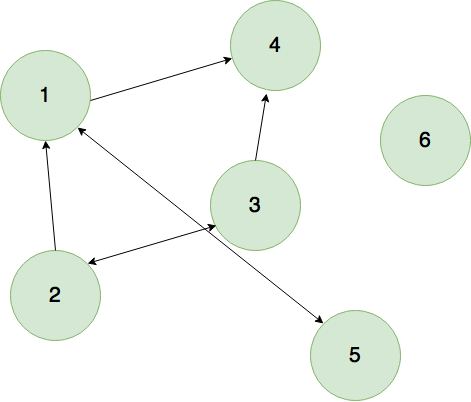
\includegraphics[width=0.4\linewidth,height=\textheight,
keepaspectratio]{Graph.png} 
\caption[Graph Example]{The picture shows  a simple example of a network with 6 Nodes. The arrows are showing the connections (links) between the different nodes. Some of the links are unidirectional, others bidirectional.}
\label{fig:simpleNetwork}
\end{figure}
Following this concept the adjacency matrix for the network in figure \ref{fig:simpleNetwork} is given by:
\begin{equation}
A = \left( \begin{matrix}
 0 & 0 & 0 & 1 & 1 & 0\\
 1 & 0 & 1 & 0 & 0 & 0\\
 0 & 1 & 0 & 1 & 0 & 0\\
 0 & 0 & 0 & 0 & 0 & 0\\
 1 & 0 & 0 & 0 & 0 & 0\\
 0 & 0 & 0 & 0 & 0 & 0
 \end{matrix}
 \right). \label{eq:adjMatExamp}
\end{equation}
Note that the matrix would be symmetric if all links were bidirectional. 
If certain links were stronger than others, one would attach so called weights to the vertices, which could for example represent the number of cows being traded from one farm to another. If the link represented by $a_{rs}$ had a strength (or weight) of $85$, this would be represented by $a_{rs}= 85$. 
\paragraph{Reachability}
One way of determining if node $k$ is reachable by node $l$ in $n$ steps is taking the $n$th power of $A$ and inspecting its entry $a_{lk}$. For example the potencies 
\begin{equation}
A^2 = \left( \begin{matrix}
 1 & 0 & 0 & 0 & 0 & 0\\
 0 & 1 & 0 & 2 & 1 & 0\\
 1 & 0 & 1 & 0 & 0 & 0\\
 0 & 0 & 0 & 0 & 0 & 0\\
 0 & 0 & 0 & 1 & 1 & 0\\
 0 & 0 & 0 & 0 & 0 & 0
 \end{matrix}
 \right),
 A^3 = \left( \begin{matrix}
 0 & 0 & 0 & 1 & 1 & 0\\
 2 & 0 & 1 & 0 & 0 & 0\\
 0 & 1 & 0 & 2 & 1 & 0\\
 0 & 0 & 0 & 0 & 0 & 0\\
 1 & 0 & 0 & 0 & 0 & 0\\
 0 & 0 & 0 & 0 & 0 & 0
 \end{matrix}
 \right) 
  \label{eq:adjMatExampPot}
\end{equation}
show the connections of all nodes within two and three steps. $A^2$ shows for example 
that node 4 can be reached from node two using one of two paths with length two each. It further shows that nodes 1, 2, 3 and 5 are connected to themselves using a way of length two. This is logical because each of them has at least one bidirectional edge.
Matrix $A^3$ however shows the paths with length three. For example two paths with length three connect node 2 with node 1. This is again due to the bidirectional edges.
To find out if connections with a length of $N$ or less between two nodes exist, one would calculate the reachability matrix
 %For example the 3rd power of matrix (\ref{eq:adjMatExamp}) would show that all nodes but nodes 6 are reachable by node 3 within 3 steps. If one would want to calculate all nodes that could be reached within $N$ or less steps, one would have to take the sum:
\begin{equation}
K_N = \sum_{n=0}^N A^n, \label{eq:reachability}
\end{equation}
with $A^0 = I$, the identity matrix. In the case of this network it would not make sense to calculate more than three potencies of $A$, since they do not change the reachability. The bidirectional edges just create circles, which add up, but no new paths are created. To avoid this and therefore to make sure that only unique paths are identified, the non-zero entries of the different reachability matrices are set to one. By comparing $K_N$ with $K_{N+1}$, one can see if new path are added. 

\paragraph{Disease Spread On Networks}
As shown in figure \ref{fig:disSpreadExampl}, a given disease can spread from one node to another in case there is a link between them. For example the disease can spread from node 3 to nodes 4 and 2 in the first time step. Node 1 will soon thereafter be infected by node 2, but not by node 4. If the structure of the network stays the same, node 6 will never be infected.
\begin{figure}[htbp]

\begin{minipage}{0.5\textwidth}
\centering
\noindent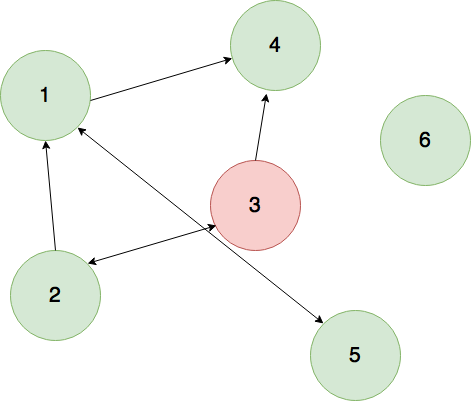
\includegraphics[width=0.9\linewidth,height=\textheight,
keepaspectratio]{Graph2.png} 
\end{minipage}
\begin{minipage}{0.5\textwidth}
\centering
\noindent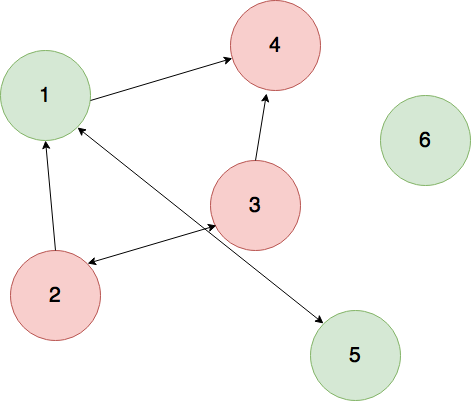
\includegraphics[width=0.9\linewidth,height=\textheight,
keepaspectratio]{Graph3.png} 
\end{minipage}
\caption[Infection Spread On A Static Network]{This picture shows the spread of a disease along the links between the nodes. Red nodes are infected, green ones are still susceptible. The third node is infected first. Nodes 4 and 2 get infected after time step 1.}
\label{fig:disSpreadExampl}
\end{figure}

\paragraph{Disease Spread on Time-dependent Networks.}
When it comes to applications for the basics discussed above, one has to find networks in real life. Unfortunately most networks in real life are not as simple and static as the examples shown above. 
If the networks changes it's structure over time, the adjacency matrix becomes time dependent:
\begin{equation}
A = A(t).
\end{equation}
This implies that the reachability in a time dependant network also changes over time and therefore depends on the start time. The potencies as described above would need to be replaced by the product of the adjacency matrix at each time:
\begin{equation}
A^n \Rightarrow \prod_{\tau=\tau_0}^{t}A(\tau).
\end{equation}
To calculate the reachability for all nodes during the time interval $\left[t_0,t\right]$ the sum over all these products as follows:
\begin{equation}
K(t,t_0) = \sum_{\tau_0 = t_0}^{t} \prod_{\tau=\tau_0}^{t}A(\tau).
\end{equation}
Figure \ref{fig:timeDependantNetworkSpread} illustrates the time dependency of disease spreading on time dependant networks. It is a sequel to the disease spreading shown in figure \ref{fig:disSpreadExampl}. It shows the state two time steps later. The yellow nodes recovered while the disease kept on spreading.
The network only changes slightly but makes it impossible for the disease to spread from node 1 to node 5. Instead it infects node 6 which would have stayed unaffected if the network would have stayed in it's earlier state. Even if the network would go back to it's earlier configuration the disease would not spread from node 1 to node 5 because node 1 will already have recovered in the next time step and therefore be unable to infect any other node. The only possibility for the disease to reach node 5 would be an upcoming link from node 6 to node 5.
\begin{figure}[htbp]
\begin{minipage}{0.5\textwidth}
\centering
\noindent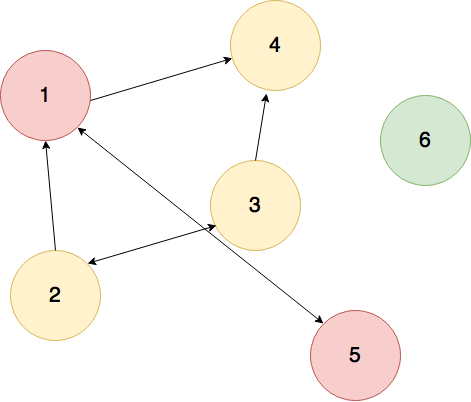
\includegraphics[width=0.9\linewidth,height=\textheight,
keepaspectratio]{Graph4.png} 
\end{minipage}
\begin{minipage}{0.5\textwidth}
\centering
\noindent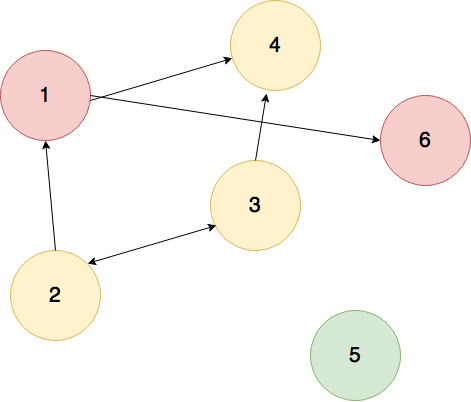
\includegraphics[width=0.9\linewidth,height=\textheight,
keepaspectratio]{Graph5.png} 
\end{minipage}
\caption[Disease Spread On A Time Dependant Network]{The two graphs show the difference a time-varying network can make for the spread of a disease on it. It is illustrating the state of the network to time steps later than in the figure \ref{fig:disSpreadExampl}. The yellow nodes are recovered. In the left hand picture node 1 infects node 5. In the picture on the right hand side node 1 infects node 6 instead. Even if the network would go back to its earlier state, node 1 would be recovered (yellow) in the next time step and therefore be unable to infect node 5. Note that node 4 cannot be infected by node 1 anymore because it had been infected earlier and became recovered and therefore immune in the mean time.}
\label{fig:timeDependantNetworkSpread}
\end{figure}


\subsection{Networks of Stochastic Oscillators}
It is possible to analytically predict the behavior of a whole system of many nodes with a basic SIR-Model, as it was shown by \citep{ROZ11}. The system described by them was a network of $n$ cities which exposed a fixed point. In contrast to the examples given above this means that the node is not either infected or susceptible as a whole, but every node is split up into different compartments. There is a probability for an individual to travel from one city to another. This leads to a statistically oscillating system. The fluctuations in the system could be described by a power spectrum derived from a Fokker-Planck equation. 
The eigenvalues of the system turn out to be quite close to the eigenvalues of a single city. The phenomenological explanation for this is that the cities behave like a single city, if the coupling and therefore the mixing is pretty strong. They behave like single cities, if the coupling is weak. 
Transferring this result on the case of BVD implies that the stable state of the whole system would be close to the stable state of a single farm. The distributions for single farms can be found in chapter \ref{chap:rlDataRegulationGermany}. However these results require a network which allows for all farms to at least get infected once. Therefore it might not be applicable to our network since some farms do not necessarily buy cows.
\section{Containment Strategies}\label{chap:containmentBasics}
This thesis focuses on containment strategies in the cattle trade network of Thuringia, one of the German federal states. This chapter will elaborate on the different methods which are used to then be used for the various strategies discussed later in the chapter.

\subsection{Methods of Containment}
In real life different mechanisms will be applied together to control a specific disease. The ones interesting in the case of BVD shall be discussed in the following few paragraphs. More or less all data about these methods have been obtained through personal communication \citep{personalCom}.

\paragraph{Individual Testing}
In general a wide variety of tests to determine if a test subject carries a certain virus exist. In the case of BVD only two different strategies are applied. They are either testing on the virus itself and its parts, (virological test) or they are testing on antibodies (serological tests) \citep{haller1999diagnostik}, \citep{personalCom}. 

\subparagraph{Virological Tests} test for parts of the virus or the virus as a whole. In case of BVD they are mostly done using the cut off material from the calf's ear when they get an ear tag, but also "normal" blood samples are taken. According to \citep{personalCom} both strategies have a sensitivity of $99.8\,\%$ and a specifity of $\approx 100\,\%$. Farmers can decide to do a second test on a cow which has been tested positive once, in order to prove that it was only a transient infection. This can only be done after 21 days for another ear tag test or 42 days later after a blood test.

\subparagraph{Serological Tests} test for antibodies. Since the body has to react to the virus first, serological tests are in general a little bit slower then virological tests and they could also react to maternal antibodies, so they are not used as often.

\paragraph{Herd Testing}
Tests on BVD for individual animals only cost a few Euros per cow but since the milk price is very low, other ways of measuring the prevalence on herd level are tested, in order to lower the financial losses. 

\subparagraph{Young Calf Window (YCW)/ Jungtierfenster (JTF))}
The YCW is a very effective way of measuring the herd prevalence. Following table 1b) from \citep{flileitfaden15}, p. 15, a minimum group of $n=14$ animals needs to be tested to determine with a certainty of $95\%$ if the prevalence in the herd is below $20\%$. Table \ref{tab:certaintyPrevalenceTest} shows the number of animals $n$ of a total population $N$ that need to be tested to prove the same prevalence with a certainty of $95\%$. After testing $n$ animals with a single positive result the prevalence has to be $p>20\%$, so that it is very likely that there is a PI in the population. After this other measures such as quarantine and tests on animals to determine their health status can follow.
\begin{wraptable}{r}{0.35\textwidth}

    \begin{center}
    \begin{tabular}{|cc|}\hline
        \rowcolor{dunkelgrau} $N$          & $n $ \\\hline
                                $\leq 10  $& $8 $ \\\hline
\rowcolor{hellgrau}             $\leq 20  $& $10$ \\\hline
                                $\leq 30  $& $11$ \\\hline
\rowcolor{hellgrau}             $\leq 60  $& $12$ \\\hline
                                $\leq 180 $& $13$ \\\hline
\rowcolor{hellgrau}             $>    180 $& $14$ \\\hline 
                              
\end{tabular}

\caption[Sample Sizes For Young Calf Window]{Number of animals $n$ of a population $N$ that need to be tested to prove with a certainty of $95\%$ that the prevalence in the herd is below $20\%$ according to \protect\citep{flileitfaden15}.}
\label{tab:certaintyPrevalenceTest} 
\end{center}
\vspace{-70pt}

\end{wraptable}
\subparagraph{Bulk Milk}
For the sake of completeness another way of measuring the prevalence of a whole herd shall be mentioned here. It is possible to measure the level of BVD-specific antibodies and therefore determine if there was a new infection event in the herd recently.
\paragraph{Removal}
Cows tested positive need to be removed from the farm. Most of the time farmers will cull them when they have been tested positive, but according to Gethmann some farmers used to sell them to other countries near by which had no restriction on BVD such as the Netherlands.

\paragraph{Quarantine}
Quarantine is a well known method used to isolate and fight diseases of all kinds. People are even discussing it in the IT sector \citep{moore2003internet}. Quarantines change the structure of the network as a whole. On the other hand it has been shown by \citep{Keeling20051} that local fluctuations in the transmission are dissipated in a very short timeframe, which is why this measure of disease control is not applied on it's own.

\subsection{Tested Strategies}
In this little section the different measures of controlling the disease spread shall be discussed.
\paragraph{Strategy I - No Measures}
In order to measure the effect that the different tested strategies are having, the first strategy examined serves just for comparison.
\paragraph{Strategy II - Old BVD Regulation}
The old BVD regulation requires are newborn calves to be tested. They should be tested immediately after their birth (when they get their eartag) and if the test result is positive, they should be removed immediately (see above). The farmer can decide to wait for another test, but many federal states decided to pay a bonus towards farmers who remove cows which were tested positive within a small time frame \citep{personalCom}. The time that has to pass for a second test depends on the kind of test (see above). The old BVD regulation offered a time frame of up to $60\,\text{days}$ to retest the cow before it had to be removed. 
If a test is negative, the mother will also be marked negative, because calves of PIs are always PIs. Cows with a positive result may not be traded.
\paragraph{Strategy III - New BVD Regulation}
The new BVD regulation limits the time span to remove a cow that has been tested positive to 40 days. Additionally the farm will be put under quarantine for this time. 
\paragraph{Strategy IV - New BVD Regulation + Vaccination}
In addition to the rules of the new BVD regulation all cows need to be vaccinated. They will be vaccinated righter after 6 months when the maternal antibodies stop working and the vaccination will be applied again every year. 
\paragraph{Strategy V - New BVD regulation + Young Calf Window}
As explained above the idea of the YCW is to test the prevalence of the whole herd. In case that one of the $n$ tested cows is tested positive, the farm has to test more cows. The rules for the whole procedure are made by the federal state. This thesis focuses on Thuringia, but the rules for Bavaria (a neighbor federal state) and Austria are given for comparison.
\subparagraph{Thuringia}\label{chap:stratThuringia}
\begin{itemize}
\item $n = 15\,\text{cows}$ need to be tested (compare to table \ref{tab:certaintyPrevalenceTest}).
\item All cows need to be older then 6 months, so that they are not protected by maternal antibodies.
\item All animals need to be unvaccinated.
\item The sample group should have the same demography as the farm as a whole.
\end{itemize}
Gethmann suggested to test all animals after a positive test of one of these tested cows, since there is no single procedure that has to be taken afterwards. While all cows are tested, the farm has to be put under quarantine. If one or more animals are found to be PIs, they have to be found immediately. Calves of cows that were pregnant during this phase need to be tested at an age of 2-6 months (compare to Bavaria' procedure). Furthermore Gethmann suggested to test two subscenarios:
\begin{itemize}
\item a) testing once a year
\item b) test every $6\,\text{months}$
\end{itemize}

\subparagraph{Bavaria}
\begin{itemize}
\item $n = 5\,\text{cows}$ need to be tested. If the stable is divided into parts, at least $n = 3\,\text{cows}$ need to be tested for every section. 
\item All animals need to be unvaccinated.
\item The tested cows need to be older then 9, but younger than $24\,\text{months}$.
\end{itemize}
If all test results are negative, all cows that have been in the farm for more than $6\,\text{months}$ are marked as non-PIs, if they did arrive in the farm below the age of $24\,\text{months}$. This test has to be repeated every $5-7\,\text{months}$.
If one of the tests is positive, all 
\begin{itemize}
\item female cows between the age of $2-24\,\text{months}$ and
\item male cows between the age of $2-9\,\text{months}$
\end{itemize}
need to be examined. Calves of pregnant cows need to be tested about 2-6 months after their birth.
\subparagraph{Austria}
\begin{itemize}
\item $n = 15\,\%\text{ of all cows}$, but at least $n = 5\,\text{young cows}$ need to be tested.
\item All cows need to be older then 6 months, so that they are not protected by maternal antibodies.
\item All animals need to be unvaccinated.
\item The tested cows need to be older then 6, but younger than $24\,\text{months}$.
\item If the herd has less then 5 animals of the age, the 5 youngest cows above the age of $6\,\text{months}$  need to be tested.
\item The difference between the oldest and youngest tested cow needs to be 4 months. 
\item All tested cows need to be part of the herd for at least 3 months.
\item Cows which have been tested positive before for antibodies do not need to be tested again.
\item If there are less then $n = 5\,\text{cows}$ to be tested, all cows which fit into this scheme need to be tested.
\end{itemize}
\paragraph{Strategy VI - New BVD regulation + Vaccination + young calf window} 
This strategy tests all the techniques discussed above.
\subsection{Mathematical Implications of Containment Strategies}
All containment strategies aim to lower the probability of infection. Since the probability of transmitting the virus in the case that two individuals meet can not be reduced, the probability of infected cows meeting susceptible cows needs to be reduced. 
Testing and culling of animals, which were tested positive, reduces the number of infected (TIs and PIs), especially the number of PIs. This is basically done by increasing the death rate of both groups. 
Quarantine changes the structure of the network. It will set at least the outgoing component of the adjacency matrix of this farm to zero, thereby reducing the probability for other farms to add a TI or PI to their farm. Unfortunately the test does not detect all infecteds, so there is still a small entry rate of PIs and TIs in every farm.
The YCW is just another way of improving the certainty that a infection in the herd is detected thereby increasing the effect of the other two methods.

\section{Real-World Results of Existing Legislation}\label{chap:rlData}
For later comparison with the results of our numerical studies some results will be presented here. 

\subsection{Prevalences without any Regulation}

\paragraph{Germany}
\subsection{Regulation in Germany}\label{chap:rlDataRegulationGermany}
\paragraph{Thuringia}
The distribution of the different compartments of a single farm with PIs which have been in this farm for some time is the following:
\\
\begin{minipage}[t]{0.5\linewidth}
No PIs
    \begin{itemize}
    \item $S= 79\,\%$
\item $I= 2\,\%$
\item $P= 0\,\%$ 
\item $R= 29\,\%$
    \end{itemize}
\end{minipage}
\begin{minipage}[t]{0.5\linewidth}
PIs for a long time
    \begin{itemize}
    \item $S= 46\,\%$
\item $I= 6\,\%$
\item $P= 2\,\%$ 
\item $R= 46\,\%$.
    \end{itemize}
\end{minipage}
\\
A survey across all of Thuringia in 2010 revealed those distributions. This survey revealed that $534\,\text{PIs}$ were living in $211\,\text{farms}(\approx 2\,\%)$. of all farms.\footnote{ (Quelle) }

\chapter{Description of the Simulation}
\section{Agent Based Simulation}
\subsection{Breeding Dynamics}
\subsection{Disease Dynamics}
\section{Farms}
\section{Disease Spread}
\section{Trading}
\section{Containment Strategies}

\chapter{Results}
In this chapter the results produced by the application of the different trading strategies are discussed, but first of all final instructions on the setup of the system are given. 
\section{Final Setup}
After the previously performed trading analysis in chapter \ref{chap:tradingDynamics} the configuration from scenario has been used in all further studies. The corresponding ini files can be found in the appendix in \ref{chap:iniContainment}. They resemble the description given in chapter \ref{chap:testedStrategiesDesc}.  
In order to keep the runtime reasonable for this thesis and testing, farms with a smaller size than 20 cows have been excluded from the simulation. The argument for this is that small farms can not build a sustainable business and are rather run by families, which want to make some money besides their daytime jobs. They will most likely not buy and sell cows all the time and therefore not play a big role in the spreading of BVD on the network. This assumption has not been proven by now. \citep{steinbach16} provided a categorisation of nodes based on their trading behavior as markets, traders, self-sustaining premises, fattening and breeding farms. This method could be refined to build a more realistic model of the market in the future. 
Applying this idea removes $15272\cows$ ($4.46\,\%$) in $5544\,\text{farms}$ ($82.16\,\%$).
Since the behavior of the different farms has not been studied and implemented in this simulation fully and because the system size in terms of farms is much smaller than the actual network size of all of Thuringia, the implementation of a more refined and realistic market behavior has been postponed. 
The data given in chapter \ref {chap:rlDataRegulationGermany} has been used to set up the system. This was done by randomly choosing $2\,\%$ of the farms to be set up with the shares of the different compartments of previously with PIs contaminated farms. The other $98\,\%$ of the farms were set up with the shares of all compartments corresponding to now previous contamination by PIs. With all these measures taken multiple simulations where run. The global prevalence strongly depends on the farms chosen to be infected in the beginning. If smaller farms are contaminated in the beginning, the disease will need much longer to spread or even die out, since far less animals are infected and the in- and out-degree of these small farms are relatively small, which leads to a smaller infection rate for all other nodes. With the aim of limiting the amount of scenarios to be discussed, one scenario which exposed a prevalence close to the big single farm with approximately $40000\cows$ from section \ref{chap:diseaseDynamicsDesc} has been chosen. It exhibited the highest global prevalence after $20\days$. The seed from this run is used in all runs for the different strategies, to make sure that the transients for the system for all strategies look exactly the same. By setting the seed of the random number generator, two streams of random numbers produced by this random number generator will be exactly the same. This is used to have the same events happen during the transient phase for all strategies, leading to results, which can be compared. The containment strategies in each scenario are turned on on a global scale after $10000\days$. The cows from the cow well farm still 
\section{Strategy I - No Strategy}
This first run corresponds to the control group in clinical tests of medication. As can be seen in figure \ref{fig:cont1Behav}, the simulation reaches a stable state with some smaller oscillations between $5000\text{ and } 10000\days$. The numbers of TIs and PIs are almost the same with the number of TIs being slightly higher, at around $1.75\,\%$ of the total population. The number of recovered animals stabilizes around $80\,\%$ of the population. The numbers of recovered and transiently infected animals are lower than they were for the single farms in chapter \ref{chap:diseaseDynamicsDesc}, whereas the prevalence of PIs is slightly higher. The number of susceptibles is much higher compared to the results for the single farm. 
\begin{figure}[htbp]
\begin{minipage}{0.5\textwidth}
\centering
\noindent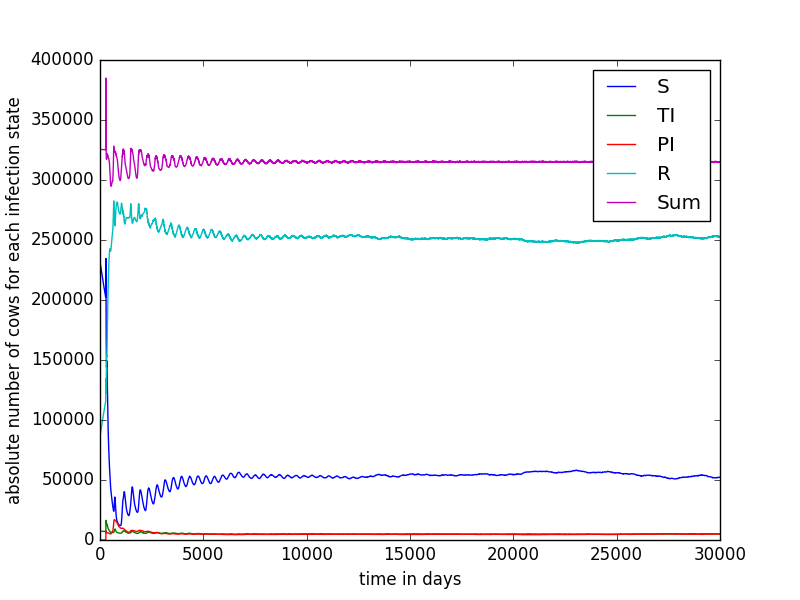
\includegraphics[width=0.95\linewidth,height=\textheight,
keepaspectratio]{cont1totalEndemicNumbers.png} 
\end{minipage}
\begin{minipage}{0.5\textwidth}
\centering
\noindent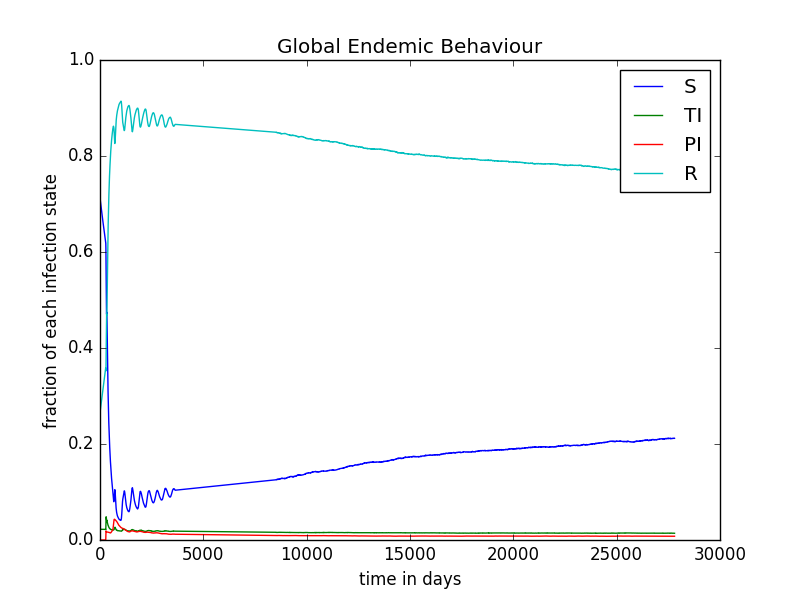
\includegraphics[width=0.95\linewidth,height=\textheight,
keepaspectratio]{cont1endemicFractions.png} 
\end{minipage}
\caption[Endemic Behavior in Containment Strategy One]{}
\label{fig:cont1Behav}
\end{figure} 

The difference in the results have to be created by the way the system is initialized. This shows that due to the way of initializing the system far less farms and therefore cows are actually reached by the disease. On the other hand this seems to increase the risk of PIs being produced if an infected animal reaches a farm of purely susceptibles, leading to a slightly higher share of PIs on the total population of the system.

\section{Strategy II - Old BVD regulation}
As described above the scenario described in this chapter will deal with tests made on every calve a few days after its birth, following the "old" German BVD regulation.
\begin{figure}[htbp]
\begin{minipage}{0.5\textwidth}
\centering
\noindent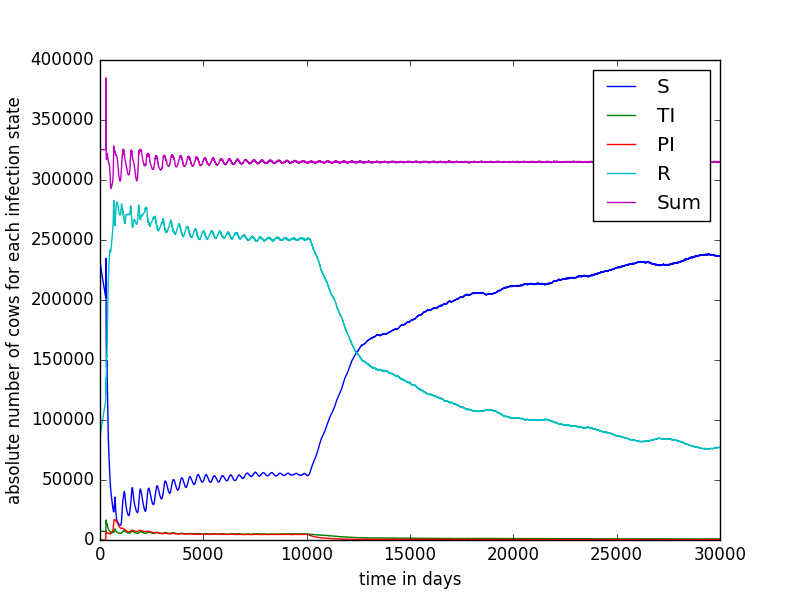
\includegraphics[width=0.95\linewidth,height=\textheight,
keepaspectratio]{cont2totalEndemicNumbers.png} 
\end{minipage}
\begin{minipage}{0.5\textwidth}
\centering
\noindent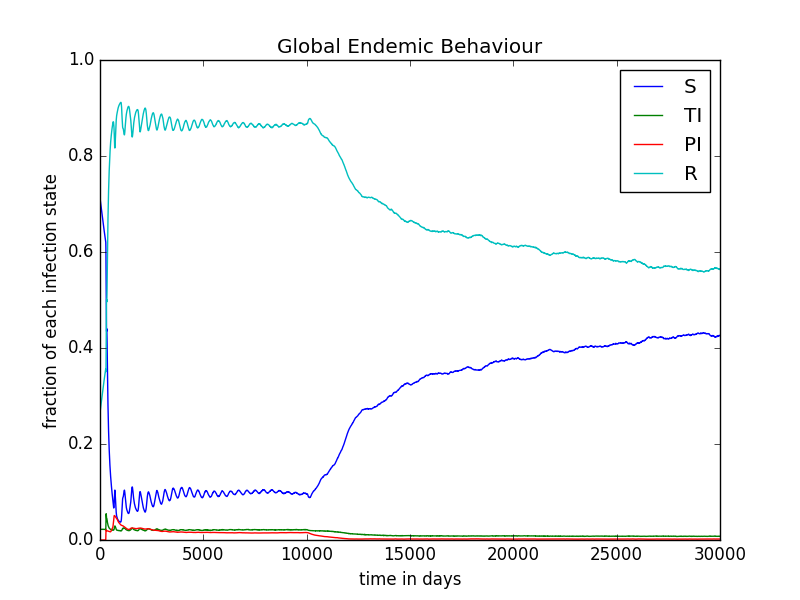
\includegraphics[width=0.95\linewidth,height=\textheight,
keepaspectratio]{cont2endemicFractions.png} 
\end{minipage}
\caption[Endemic Behavior in Containment Strategy One]{}
\label{fig:demographyScen8}
\end{figure}


\section{Strategy III - New BVD regulation}

\begin{figure}[htbp]
\begin{minipage}{0.5\textwidth}
\centering
\noindent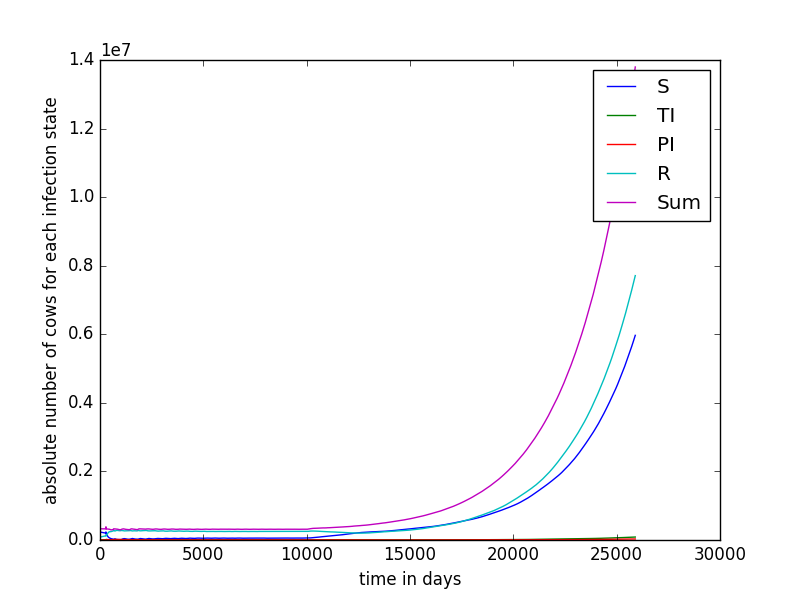
\includegraphics[width=0.95\linewidth,height=\textheight,
keepaspectratio]{cont3totalEndemicNumbers.png} 
\end{minipage}
\begin{minipage}{0.5\textwidth}
\centering
\noindent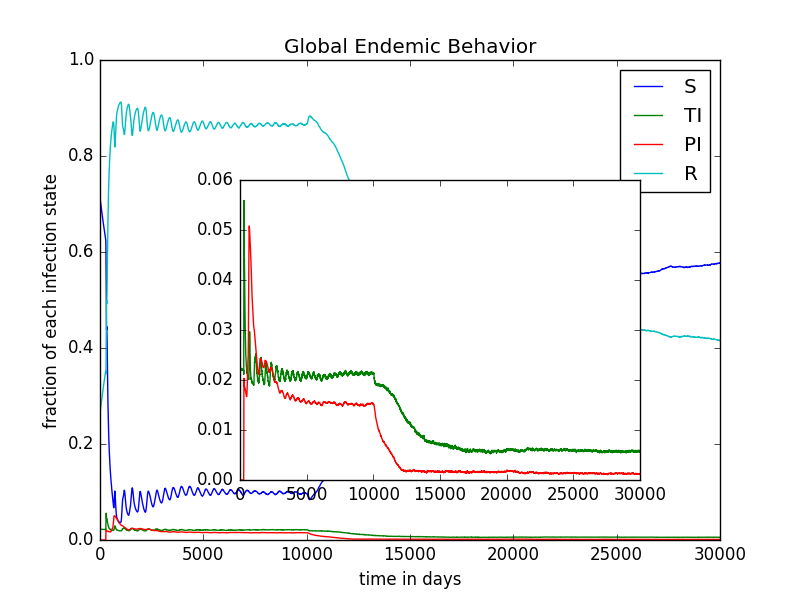
\includegraphics[width=0.95\linewidth,height=\textheight,
keepaspectratio]{cont3pendemicFractions.png} 
\end{minipage}
\caption[Endemic Behavior in Containment Strategy One]{}
\label{fig:demographyScen8}
\end{figure}


\section{Strategy IV - New BVD regulation + Vaccination}


\begin{figure}[htbp]
\begin{minipage}{0.5\textwidth}
\centering
\noindent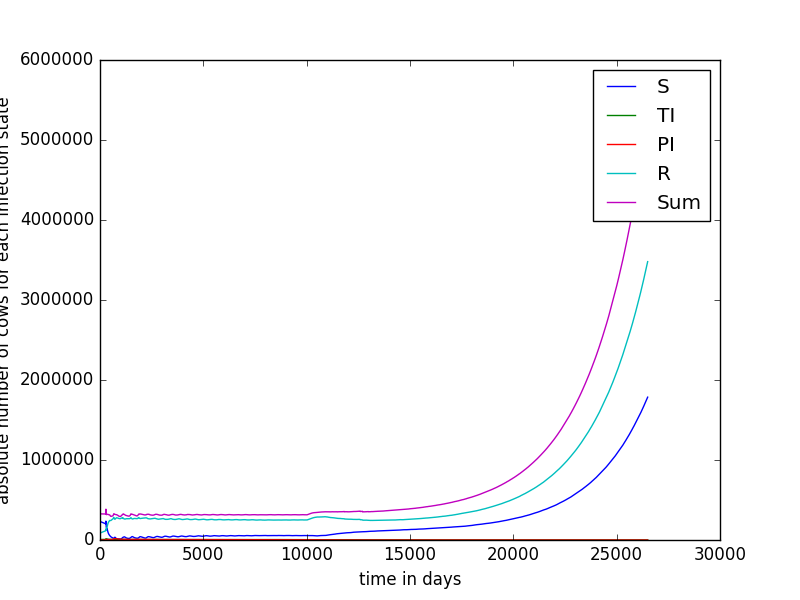
\includegraphics[width=0.95\linewidth,height=\textheight,
keepaspectratio]{cont4totalEndemicNumbers.png} 
\end{minipage}
\begin{minipage}{0.5\textwidth}
\centering
\noindent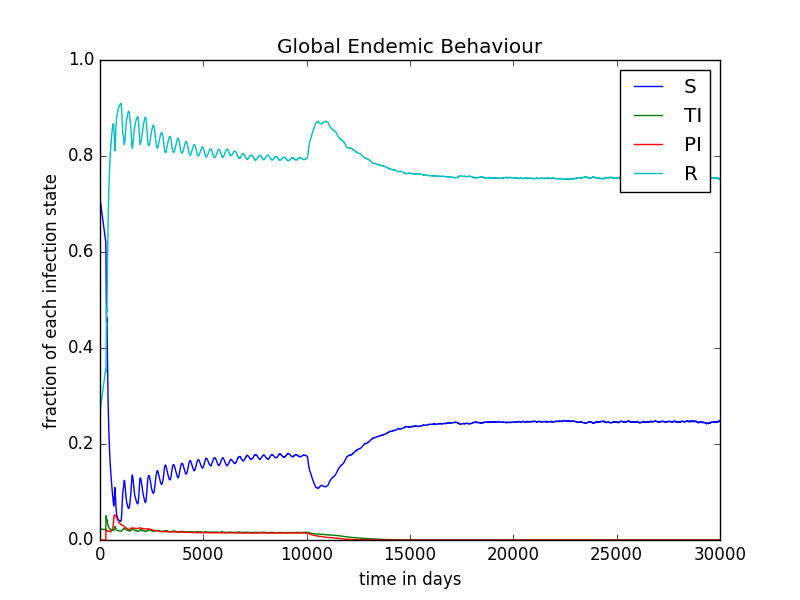
\includegraphics[width=0.95\linewidth,height=\textheight,
keepaspectratio]{cont4endemicFractions.png} 
\end{minipage}
\caption[Endemic Behavior in Containment Strategy One]{}
\label{fig:demographyScen8}
\end{figure}


\section{Strategy V - New BVD regulation + young calf window}
\subsection{Strategy Va}

\begin{figure}[htbp]
\begin{minipage}{0.5\textwidth}
\centering
\noindent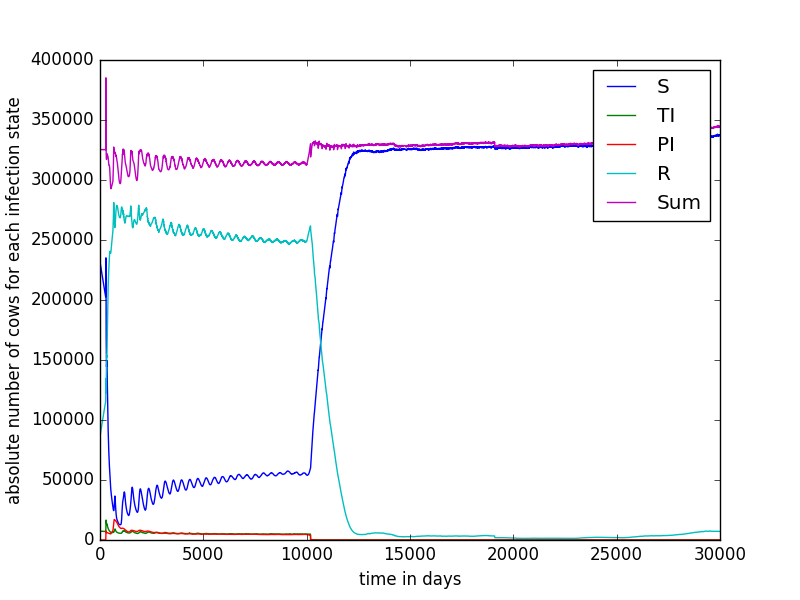
\includegraphics[width=0.95\linewidth,height=\textheight,
keepaspectratio]{cont5totalEndemicNumbers.png} 
\end{minipage}
\begin{minipage}{0.5\textwidth}
\centering
\noindent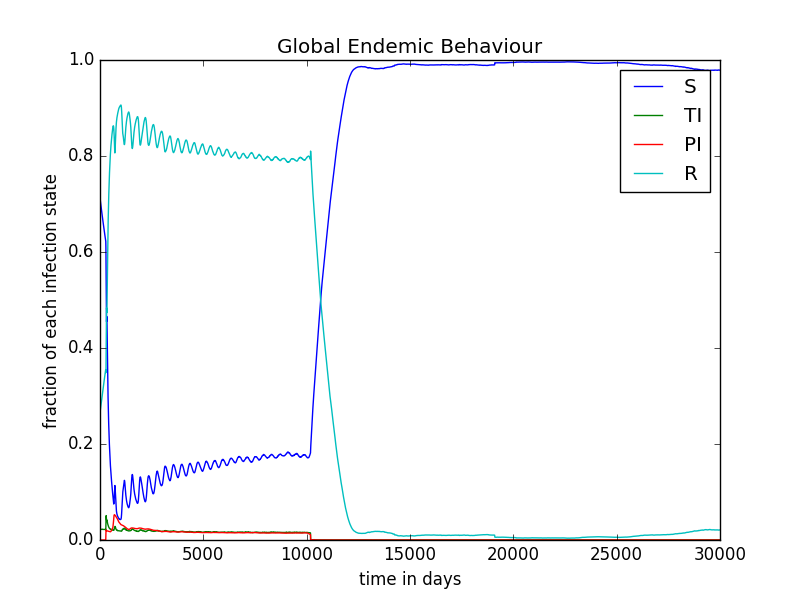
\includegraphics[width=0.95\linewidth,height=\textheight,
keepaspectratio]{cont5endemicFractions.png} 
\end{minipage}
\caption[Endemic Behavior in Containment Strategy One]{}
\label{fig:demographyScen8}
\end{figure}

\subsection{Strategy Vb}

\begin{figure}[htbp]
\begin{minipage}{0.5\textwidth}
\centering
\noindent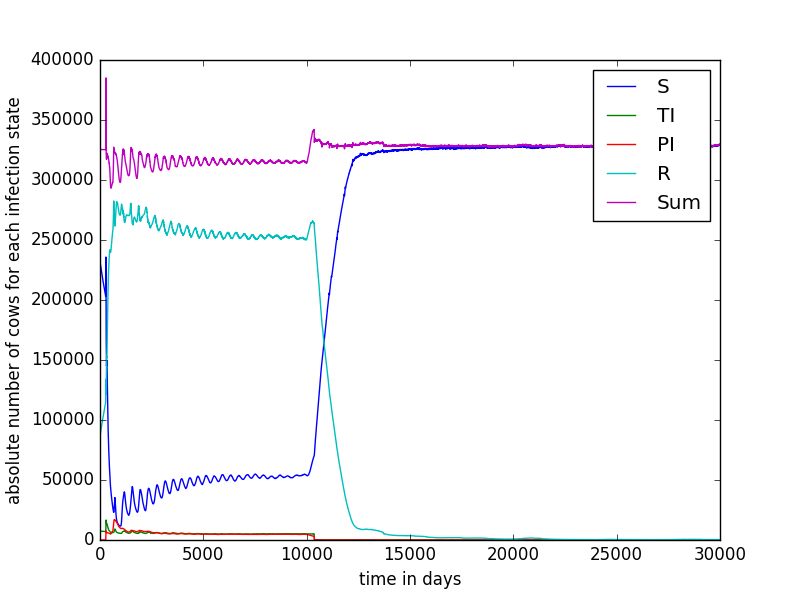
\includegraphics[width=0.95\linewidth,height=\textheight,
keepaspectratio]{cont5btotalEndemicNumbers.png} 
\end{minipage}
\begin{minipage}{0.5\textwidth}
\centering
\noindent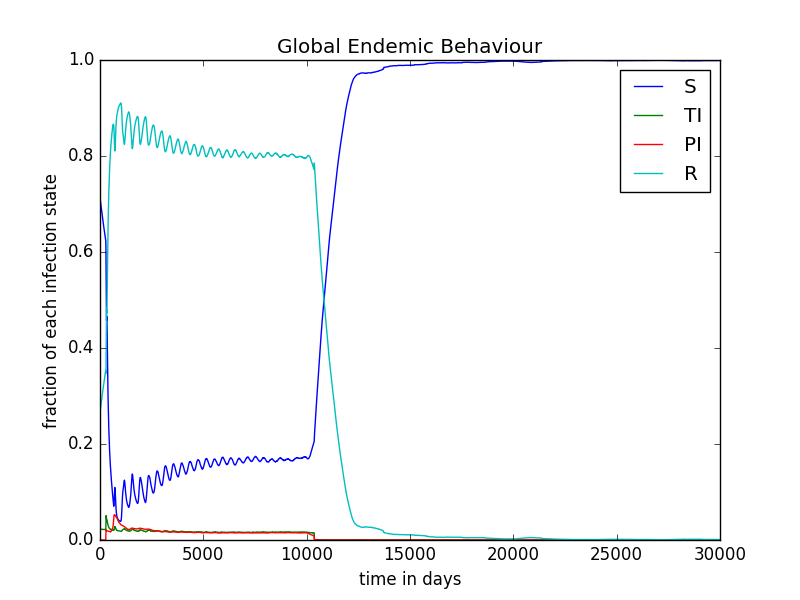
\includegraphics[width=0.95\linewidth,height=\textheight,
keepaspectratio]{cont5bendemicFractions.png} 
\end{minipage}
\caption[Endemic Behavior in Containment Strategy One]{}
\label{fig:demographyScen8}
\end{figure}

\section{Strategy VI - New BVD regulation + Vaccination + young calf window} 
\subsection{Strategy VIa}

\begin{figure}[htbp]
\begin{minipage}{0.5\textwidth}
\centering
\noindent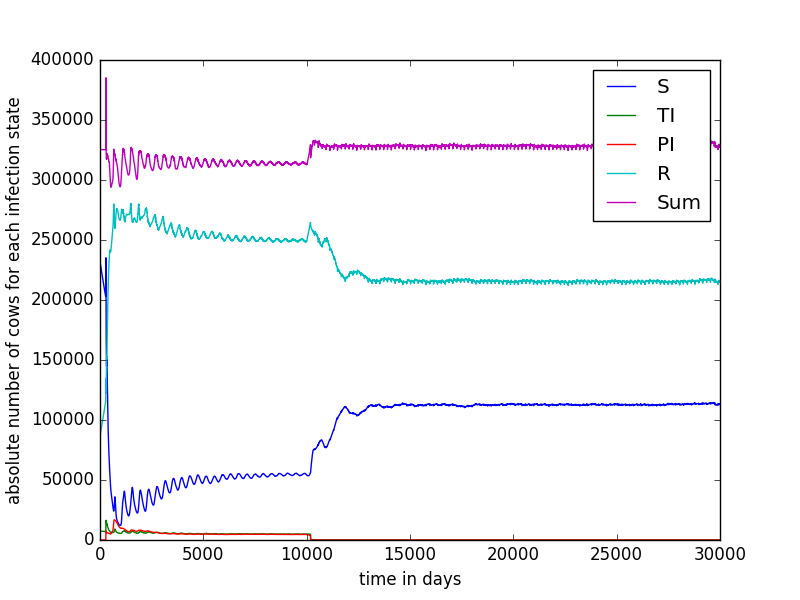
\includegraphics[width=0.95\linewidth,height=\textheight,
keepaspectratio]{cont6totalEndemicNumbers.png} 
\end{minipage}
\begin{minipage}{0.5\textwidth}
\centering
\noindent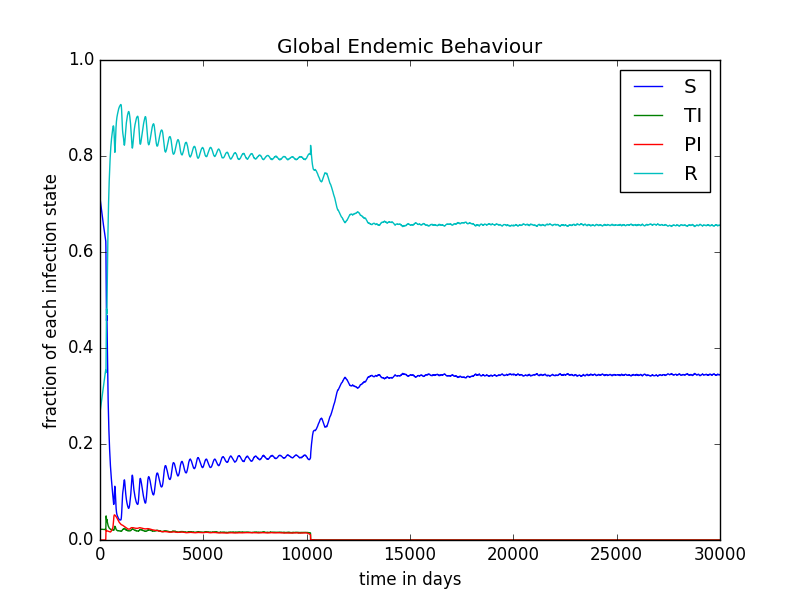
\includegraphics[width=0.95\linewidth,height=\textheight,
keepaspectratio]{cont6endemicFractions.png} 
\end{minipage}
\caption[Endemic Behavior in Containment Strategy One]{}
\label{fig:demographyScen8}
\end{figure}

\subsection{Strategy VIb}

\begin{figure}[htbp]
\begin{minipage}{0.5\textwidth}
\centering
\noindent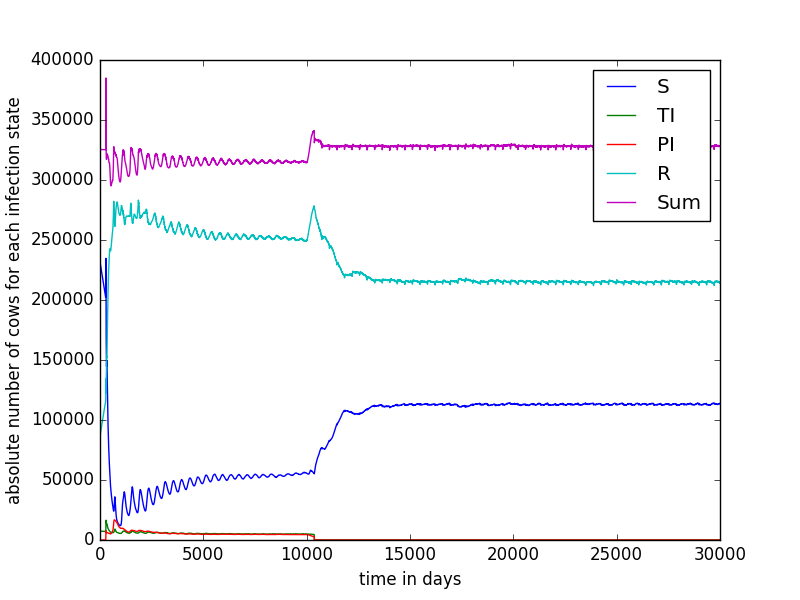
\includegraphics[width=0.95\linewidth,height=\textheight,
keepaspectratio]{cont6btotalEndemicNumbers.png} 
\end{minipage}
\begin{minipage}{0.5\textwidth}
\centering
\noindent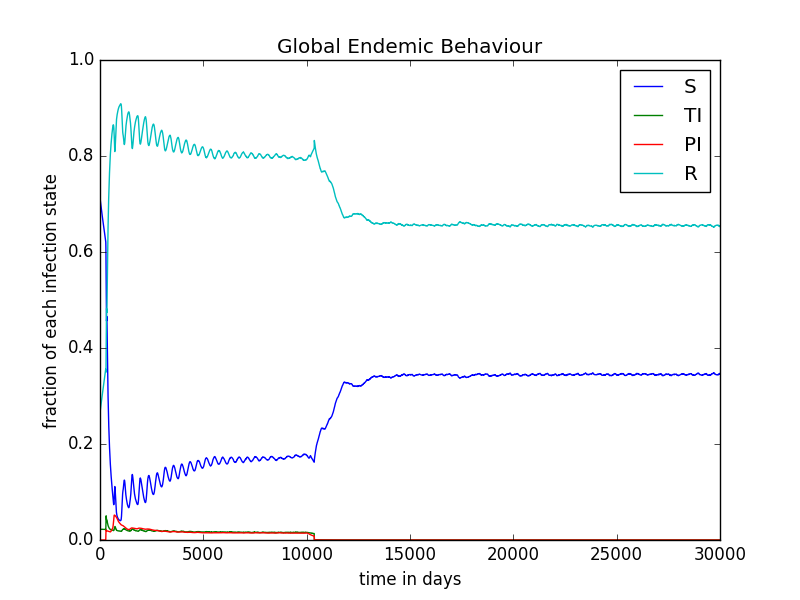
\includegraphics[width=0.95\linewidth,height=\textheight,
keepaspectratio]{cont6bendemicFractions.png} 
\end{minipage}
\caption[Endemic Behavior in Containment Strategy One]{}
\label{fig:demographyScen8}
\end{figure}

\section{Comparison of the different Strategies}
\chapter{Conclusion \& Outlook}

\section*{Acknowledgements}

\section*{Erklärung zur selbstständigen Ausarbeitung}
Hiermit erkläre ich, dass ich die vorliegende Arbeit selbstständig und eigenhändig sowie ohne unerlaubte fremde Hilfe und ausschließlich unter Verwendung der aufgeführten Quellen und Hilfsmittel angefertigt habe.
\\\\\\\
Pascal Blunk, Berlin, den \today
\appendix
\chapter{Distributions}
\section{Breeding Dynamics}
\section{Disease Dynamics}\label{appendix:diseasesistributions}

\chapter{Ini Files}
\section{Trading Scenarios}
\section{Containment Strategies}\label{chap:iniContainment}


%%%%%%%%%%%%%%%%%%%%%%%%%%%%%%%%%%%%%%%%%%%%%%%%%%%%%%%%%%%%%%%%%%%%%%%%%%%%%%%
%%%%%%%%%%%%%%%%%%%%%%%%%%%%%%%%%%%%%%%%%%%%%%%%%%%%%%%%%%%%%%%%%%%%%%%%%%%%%%%
\bibliographystyle{DEapalike} 
\bibliography{bachelor}
\end{document} 